\documentclass[a4paper,11pt]{article}
\usepackage[a4paper,bindingoffset=0in,left=0.9in,right=0.9in,top=1in,bottom=1in,footskip=.25in]{geometry}
\usepackage{generic}
\usepackage{comment}
\usepackage{graphicx}
\usepackage{epstopdf}
\usepackage{amsmath, amsthm}
\usepackage{setspace}
% Standard IEEE citation
\usepackage{cite}
 \usepackage{cuted}
%\usepackage[ruled,vlined]{algorithm2e}
 \usepackage{flushend}
 %\usepackage{multicol}
% Hyperlinks for references, URLs, sections
\usepackage[colorlinks=true, linkcolor=blue, citecolor=blue, urlcolor=blue]{hyperref}
\newtheorem{theorem}{Theorem}[section]
\newtheorem{proposition}{Proposition}[section]
\newtheorem{remark}{Remark}[section]
\newtheorem{lemma}{Lemma}[section]
% Math and symbols
\usepackage{amsmath,amssymb,amsfonts}
\usepackage{enumitem}
\setlist{noitemsep, topsep=0pt}

% Graphics
\usepackage{graphicx}
\setlength{\parindent}{0pt}
\usepackage[justification=centering]{caption}
% Algorithms
\usepackage{algorithm,algorithmic}
% \usepackage{enumerate}
\usepackage{rotating}
% Cross-referencing
\usepackage[capitalize]{cleveref}
\crefname{section}{Sec.}{Secs.}
\Crefname{section}{Section}{Sections}
\Crefname{table}{Table}{Tables}
\crefname{table}{Tab.}{Tabs.}

\def\BibTeX{{\rm B\kern-.05em{\sc i\kern-.025em b}\kern-.08em
    T\kern-.1667em\lower.7ex\hbox{E}\kern-.125emX}}


\title{Classical and Bayesian Estimation of the Lomax Distribution under Joint Improved Adaptive Progressive Censored Competing Risks Data}
\author{Ruttala Vamsi Krishna (250150034) \& Bagadi Bhargav (250150009) \\ Mehta Family School of Data Science and Artificial Intelligence, IIT Guwahati, India \\ DA2141: Statistics for Data Science --- Course Project}
\date{}
\emergencystretch=3em
\begin{document}

\begin{singlespace}
 \maketitle
\end{singlespace}

\begin{abstract}
\noindent In this article, we consider the classical and Bayesian estimation of the Lomax distribution when two production lines are tested together under a joint improved adaptive progressive Type-II censoring scheme (JIAPCS) and every failure is recorded with its cause (two independent causes per line). We write down the likelihood, show that it splits by population, and derive the maximum likelihood estimators (MLEs): the two shape parameters have closed forms for a given scale parameter, a finite MLE of the scale parameter exists under a simple sample condition (otherwise the likelihood is maximised in the exponential limit), and an order-restricted MLE for $\alpha_{d1}\le\alpha_{d2}$ is obtained in closed form. Bayes estimates under squared-error, LINEX and general-entropy losses, and HPD credible intervals, are computed without and with the order restriction using a collapsed Metropolis--Gibbs sampler. The performance of different estimators is evaluated through extensive numerical simulations (1000 replications per scenario) in terms of mean-squared error and absolute bias, while ACI and HPD credible intervals are assessed in terms of average width and coverage probability. We find that the Lomax MLE exists in only 51--79\% of the samples and is unstable when it does, that proper-prior Bayes estimates are far more accurate, and that the order restriction helps little when true but hurts when violated. Finally, two real data sets (aircraft air-conditioning failures and electrical appliances) are analyzed for illustration purposes; both are close to exponential, which shows the limits of the Lomax model.\\
\textbf{Keywords:} Lomax distribution; competing risks; joint progressive censoring; gamma prior; maximum likelihood estimator; Bayesian estimation.\\
\end{abstract}

\section{Introduction}
\label{sec:introduction}
Reliability testing is one of the important methods to assess the failure pattern of different products. In such situations, items are put on test under some operational condition and then failure times are recorded. A unit can often fail for more than one reason (for example a compressor fault or any other fault in an air-conditioning unit). The causes compete: we see only the first one that acts, together with its identity. This is the competing risks model, which goes back to Cox \cite{cox1959}; for the Lomax lifetime under progressive censoring see Cramer and Schmiedt \cite{cramer2011}.

Life tests are costly, so they are stopped early. In progressive Type-II censoring a fixed number of surviving units is withdrawn at each failure. To compare the products of two production lines, one can use both samples in a single test. Balakrishnan and Rasouli \cite{balakrishnan2008} proposed joint progressive censoring, and Mondal and Kundu \cite{mondal2019} introduced the balanced version (BJPCS), in which both samples lose the same number of units after every failure. Chen and Gui \cite{chen2026} studied BJPCS with competing risks for the Burr-XII distribution, and this is the paper our project follows. A weakness of progressive schemes is that the test can last very long. Ng, Kundu and Chan \cite{ng2009} let the scheme adapt after a time threshold $T_1$, and Yan, Li and Yu \cite{yan2021} added a second, hard deadline $T_2$; this is the improved adaptive scheme. Competing risks under improved adaptive censoring have been studied for several lifetime models (see e.g.\ \cite{alotaibi2025}), but we did not find a treatment for the Lomax distribution, nor for the two-population (joint) version of the scheme.

The Lomax (Pareto II) distribution \cite{lomax1954} has the decreasing hazard $h(x)=\alpha\lambda/(1+\lambda x)$ and a heavy tail, which suits products with early failures. It contains the exponential distribution as the limit $\alpha\to\infty$, $\lambda\to0$ with $\alpha\lambda$ fixed, and this limit will turn out to matter a lot.

\textbf{Contributions.} (i) We formulate the likelihood of the Lomax competing risks model under JIAPCS. (ii) We obtain the MLEs, with and without the order restriction $\alpha_{d1}\le\alpha_{d2}$, and study when they exist. (iii) We derive Bayes estimates under three loss functions and HPD intervals, with independent gamma priors and with the truncated (order-restricted) prior. (iv) We compare everything by simulation and (v) apply it to two real data sets. Along the way we try to derive the main results from scratch using only tools from the course (MLE, Fisher information, Cram\'er--Rao, likelihood ratio tests, Bayes estimators under a loss function; see e.g.\ Casella and Berger \cite{casella2002}).

The organization of the paper is as follows. The model, the censoring scheme and the likelihood are set up in Section~\ref{sec2}, which also gives the maximum likelihood estimators, their existence, the order-restricted MLE and the interval estimates. Bayesian estimation, with and without the order restriction, is developed in Section~\ref{sec3}. Section~\ref{sec5} presents a simulation study and two real data applications. Finally, the conclusion is given in Section~\ref{sec6}.

\section{Maximum Likelihood Estimation}\label{sec2}
\paragraph{Model.} Population $\Omega_d$ ($d=1,2$) has $m_d$ units. Each unit has two latent lifetimes $W_{d1},W_{d2}$, independent, with
\[
S_{dr}(x)=(1+\lambda_d x)^{-\alpha_{dr}},\qquad h_{dr}(x)=\frac{\alpha_{dr}\lambda_d}{1+\lambda_d x},\qquad x>0,\ r=1,2 .
\]
The two causes in a population share the scale-type parameter $\lambda_d$ but may have different shapes. This common-$\lambda_d$ assumption is what makes the algebra below work. A unit fails at $\min(W_{d1},W_{d2})$, whose survival function is $S_d(x)=(1+\lambda_dx)^{-(\alpha_{d1}+\alpha_{d2})}$ (multiply the two survival functions). Because $h_{d1}/(h_{d1}+h_{d2})=\alpha_{d1}/(\alpha_{d1}+\alpha_{d2})$ does not depend on $x$, the cause is $r$ with probability $\alpha_{dr}/(\alpha_{d1}+\alpha_{d2})$, independently of the failure time. The six unknowns are $\theta=(\alpha_{11},\alpha_{12},\lambda_1,\alpha_{21},\alpha_{22},\lambda_2)$.

\paragraph{The JIAPCS.} Fix $k<\min(m_1,m_2)$, removal numbers $R_1,\dots,R_{k-1}\ge0$ with $\sum_{i<k}(R_i+1)<\min(m_1,m_2)$, and thresholds $T_1<T_2$. Both samples are put on test together. At the $i$-th failure, at time $w_{(i)}$, in population $\Omega_z$:
(1) (adaptive rule) the number of withdrawals is $R_i$ if $w_{(i)}<T_1$ and $0$ if $w_{(i)}\ge T_1$;
(2) (balanced rule) $R_i$ survivors are withdrawn at random from $\Omega_z$ and $R_i+1$ from the other population, so both populations lose $R_i+1$ units;
(3) (improved rule) the test ends at the $k$-th failure, or at $T_2$ if fewer than $k$ failures have happened by then; all survivors are withdrawn at the end.
Three cases occur: I ($w_{(k)}<T_1$, the ordinary balanced scheme), II ($T_1\le w_{(k)}<T_2$, removals stop after $T_1$) and III ($w_{(k)}\ge T_2$, the test is stopped at $T_2$ with fewer than $k$ failures). The data are the failure times together with the population and cause of each failure.

\paragraph{Likelihood.} Let $t_{(1)}<\dots<t_{(K)}$ be the event times of the test (failure times and the final time) and let $\nu_{dj}$ be the number of $\Omega_d$ units that fail or are withdrawn at $t_{(j)}$, so $\sum_j\nu_{dj}=m_d$. Let $x_{d1},\dots,x_{dN_d}$ be the failure times in $\Omega_d$ with causes $\delta_{di}\in\{1,2\}$, and $N_{dr}=\#\{i:\delta_{di}=r\}$, $N_d=N_{d1}+N_{d2}$. A unit that fails at $x$ from cause $r$ contributes $f_{dr}(x)S_{dr'}(x)=h_{dr}(x)S_d(x)$ (cause $r$ acts at $x$ and the other cause has not yet acted). A withdrawn unit at $t$ contributes $S_d(t)$. The decisions of the scheme depend only on the past, so they are non-informative and the likelihood is proportional to the product of these terms. Taking logs and collecting the survival factors of failed and withdrawn units in $\nu_{dj}$,
\begin{equation}\label{eq:ll}
\ell_d=N_{d1}\ln\alpha_{d1}+N_{d2}\ln\alpha_{d2}+N_d\ln\lambda_d-\sum_{i=1}^{N_d}\ln(1+\lambda_dx_{di})-(\alpha_{d1}+\alpha_{d2})D_d(\lambda_d),
\end{equation}
where $D_d(\lambda)=\sum_{j=1}^{K}\nu_{dj}\ln(1+\lambda t_{(j)})$. The full log-likelihood is $\ell_1+\ell_2$ and the two parts share no parameters, so $\Omega_1$ and $\Omega_2$ are analysed separately with the same three-parameter routine. From now on we drop the index $d$.

\subsection{MLE Under no order restriction}
\begin{theorem}[Shape parameters]\label{thm:shape}
For fixed $\lambda$ and $N_1,N_2\ge1$, $\ell$ is maximised by $\hat\alpha_r(\lambda)=N_r/D(\lambda)$, $r=1,2$.
\end{theorem}
\begin{proof}
As a function of the shapes, $\ell=\sum_rN_r\ln\alpha_r-(\alpha_1+\alpha_2)D+\text{const}$. Setting $\partial\ell/\partial\alpha_r=N_r/\alpha_r-D=0$ gives $\hat\alpha_r=N_r/D$, and $\partial^2\ell/\partial\alpha_r^2=-N_r/\alpha_r^2<0$ shows it is a maximum.
\end{proof}
Substituting back gives the profile log-likelihood of $\lambda$ (up to a constant),
\begin{equation}\label{eq:prof}
\ell_p(\lambda)=N\ln\lambda-\sum_{i=1}^{N}\ln(1+\lambda x_i)-N\ln D(\lambda),
\end{equation}
with score $\ell_p'(\lambda)=N/\lambda-\sum_i x_i/(1+\lambda x_i)-N D'(\lambda)/D(\lambda)$ and $D'(\lambda)=\sum_j\nu_jt_{(j)}/(1+\lambda t_{(j)})$.

\begin{theorem}[Existence of $\hat\lambda$]\label{thm:exist}
Let $S_1=\sum_ix_i$, $W=\sum_j\nu_jt_{(j)}$, $Q=\sum_j\nu_jt_{(j)}^2$ and $\Psi=NQ/(2W)-S_1$. If $\Psi>0$, then $\ell_p$ has a maximum at a finite $\hat\lambda\in(0,\infty)$ which solves $\ell_p'(\lambda)=0$, and $\hat\alpha_r=N_r/D(\hat\lambda)$ are the MLEs. If $\ell_p$ is maximised only at the boundary, the supremum of the likelihood is approached as $\lambda\to0$ with $\alpha_r\to\infty$ and $\alpha_r\lambda\to N_r/W$, i.e.\ by the exponential competing risks model.
\end{theorem}
\begin{proof}
\emph{(a) Behaviour near $0$.} Use $\ln(1+u)=u-u^2/2+O(u^3)$. Then $D(\lambda)=\lambda W-\tfrac12\lambda^2Q+O(\lambda^3)$, so
$\ln D=\ln\lambda+\ln W+\ln\!\big(1-\tfrac{\lambda Q}{2W}+O(\lambda^2)\big)=\ln\lambda+\ln W-\tfrac{\lambda Q}{2W}+O(\lambda^2)$, and $\sum_i\ln(1+\lambda x_i)=\lambda S_1+O(\lambda^2)$. Putting these into \eqref{eq:prof}, the $N\ln\lambda$ terms cancel and
\[
\ell_p(\lambda)=-N\ln W+\lambda\Big(\frac{NQ}{2W}-S_1\Big)+O(\lambda^2)=-N\ln W+\lambda\Psi+O(\lambda^2).
\]
So $\ell_p'(0+)=\Psi$, and if $\Psi>0$ the profile is increasing near $0$.
\emph{(b) Behaviour at $\infty$.} $N\ln\lambda-\sum\ln(1+\lambda x_i)=-\sum\ln(x_i+1/\lambda)\to-\sum\ln x_i$ is finite, while $D(\lambda)\ge\ln(1+\lambda t_{(1)})\to\infty$ (the weights $\nu_j$ add up to $m>0$). Hence $-N\ln D\to-\infty$ and $\ell_p\to-\infty$.
\emph{(c)} $\ell_p$ is continuous on $(0,\infty)$, starts above its limit $-N\ln W$ (by (a)) and goes to $-\infty$ (by (b)), so it has a global maximum at an interior point where $\ell_p'=0$.
For the boundary statement let $\lambda\to0$ with $\alpha_r\lambda=\kappa_r$ fixed. Then $(1+\lambda x)^{-\alpha_r}\to e^{-\kappa_rx}$, $\sum\ln(1+\lambda x_i)\to0$, $(\alpha_1+\alpha_2)D\to(\kappa_1+\kappa_2)W$, so \eqref{eq:ll} tends to $\sum_rN_r\ln\kappa_r-(\kappa_1+\kappa_2)W$, which is the exponential competing risks log-likelihood and is maximised at $\kappa_r=N_r/W$.
\end{proof}

\begin{remark}[About uniqueness and non-existence]
$\Psi>0$ is only a sufficient condition in the proof. For a complete sample ($\nu_j=1$, $W=S_1$) it reads $\overline{x^2}>2\bar x^{2}$, i.e.\ the squared coefficient of variation is larger than $1$; so the Lomax likelihood needs a clearly heavy-tailed sample. We could not prove uniqueness of the root, so we checked it numerically: in 1000 simulated samples (design D2, ``mid'' pattern, thresholds PB, $\Omega_1$) none had two or more interior maxima of $\ell_p$, $65.7\%$ had exactly one and $34.3\%$ had none, and the event $\{\Psi>0\}$ coincided with the event that a finite MLE exists. So in practice $\Psi>0$ is necessary and sufficient and the root is unique. A claim of a unique finite MLE for every sample would be wrong: when $\Psi\le0$ the MLE does not exist (flat profile, \cref{fig:real1}(a)).
\end{remark}

\paragraph{Computation.} We evaluate $\ell_p$ on a log-grid of 400 values of $\lambda$ around $N/W$, take the grid maximum and refine the root of $\ell_p'$ by bisection (60 steps). If the grid maximum is on the boundary we declare that the MLE does not exist.

\begin{remark}[A check in the simplest case]\label{rem:umvue}
Take one cause, a complete sample of size $n$ and known $\lambda$. Then $Y=\ln(1+\lambda X)$ satisfies $P(Y>y)=P\big(X>(e^y-1)/\lambda\big)=e^{-\alpha y}$, so $Y\sim\mathrm{Exp}(\alpha)$ and $T=\sum_iY_i\sim\mathrm{Gamma}(n,\alpha)$ (rate $\alpha$); $T$ is sufficient and complete, and the MLE is $\hat\alpha=n/T$. Since $E(1/T)=\alpha/(n-1)$, we get $E\hat\alpha=n\alpha/(n-1)$: the MLE is biased in small samples. The estimator $\tilde\alpha=(n-1)/T$ is unbiased and a function of a complete sufficient statistic, hence the UMVUE (Lehmann--Scheff\'e) with $\mathrm{Var}(\tilde\alpha)=\alpha^2/(n-2)$, which is slightly above the Cram\'er--Rao bound $\alpha^2/n$ (the bound is not attained). A simulation with $n=10$, $\alpha=0.8$, $\lambda=1.5$ ($2\times10^5$ replications) gave mean $0.889$ for $\hat\alpha$ (theory $0.889$) and mean $0.800$, variance $0.0796$ for $\tilde\alpha$ (theory $0.0800$). Moreover $\alpha T\sim\mathrm{Gamma}(n,1)$ is a pivot, which gives the exact interval $\big[\chi^2_{2n,0.025}/(2T),\ \chi^2_{2n,0.975}/(2T)\big]$, and by monotone likelihood ratio the UMP test of $H_0:\alpha\le\alpha_0$ against $H_1:\alpha>\alpha_0$ rejects for small $T$. Under JIAPCS the role of $T$ is played by $D(\lambda)$, which explains the form $N_r/D$ in Theorem~\ref{thm:shape}, but $D$ is no longer exactly Gamma (the event times are order statistics of the pooled test), so we use asymptotic and bootstrap intervals below.
\end{remark}

\subsection{MLE Under order restriction}
Often one cause is known (or believed) to be the more dangerous one, so we impose $\alpha_{d1}\le\alpha_{d2}$.
\begin{theorem}[Restricted MLE]\label{thm:restr}
Under $\alpha_1\le\alpha_2$ the restricted MLEs are
\[
\hat\alpha_1^{R}=\frac{\min(N_1,N/2)}{D(\hat\lambda)},\qquad \hat\alpha_2^{R}=\frac{\max(N_2,N/2)}{D(\hat\lambda)},
\]
with the same $\hat\lambda$ as in the unrestricted case. So the restricted estimate equals the unrestricted one if $N_1\le N_2$, and pools the two shapes to $N/(2D(\hat\lambda))$ otherwise.
\end{theorem}
\begin{proof}
Fix $\lambda$ and write $g(\alpha_1,\alpha_2)=N_1\ln\alpha_1+N_2\ln\alpha_2-(\alpha_1+\alpha_2)D$, a concave function with unrestricted maximiser $(N_1,N_2)/D$. If $N_1\le N_2$ this point satisfies $\alpha_1\le\alpha_2$, so it is also the restricted maximiser. If $N_1>N_2$ it lies outside the convex region $\{\alpha_1\le\alpha_2\}$, and the maximum of a concave function over a convex region is then on the boundary $\alpha_1=\alpha_2=\alpha$, where $g=N\ln\alpha-2\alpha D$ is maximised at $\alpha=N/(2D)$. In both cases the maximised value is $-N\ln D$ plus a quantity free of $\lambda$ (it equals $\sum N_r\ln N_r-N$ or $N\ln(N/2)-N$), so the profile in $\lambda$ is \eqref{eq:prof} up to a constant and has the same maximiser $\hat\lambda$. The compact form follows from $\min(N_1,N/2)$ and $\max(N_2,N/2)$.
\end{proof}

\paragraph{Is the restriction plausible? A likelihood ratio test.} To test $H_0:\alpha_1=\alpha_2$ against $\alpha_1\ne\alpha_2$, note from the proof above that both fits have the same $\hat\lambda$, so the maximised log-likelihoods differ only through the $\alpha$-part:
\[
\Lambda=2\Big[N_1\ln N_1+N_2\ln N_2-N\ln(N/2)\Big]=2\Big[N_1\ln\frac{2N_1}{N}+N_2\ln\frac{2N_2}{N}\Big],
\]
which does not depend on $\lambda$ and is asymptotically $\chi^2_1$ under $H_0$ (Wilks). It is just the likelihood ratio test of ``$p=1/2$'' for the binomial cause counts, as it should be, since the cause is independent of the time. We use it in \cref{sec:real}.

\subsection{Interval estimation}
For $\vartheta=(\alpha_1,\alpha_2,\lambda)$ the observed information is minus the Hessian of \eqref{eq:ll}. Differentiating twice, using $D''(\lambda)=-E(\lambda)$ with $E=\sum_j\nu_jt_{(j)}^2/(1+\lambda t_{(j)})^2$,
\[
I(\hat\vartheta)=\begin{bmatrix}
N_1/\hat\alpha_1^2&0&D'\\
0&N_2/\hat\alpha_2^2&D'\\
D'&D'&\dfrac{N}{\hat\lambda^2}-\sum_i\dfrac{x_i^2}{(1+\hat\lambda x_i)^2}-(\hat\alpha_1+\hat\alpha_2)E
\end{bmatrix}.
\]
We checked these formulas against numerical second differences (maximum difference $4.5\times10^{-6}$). By asymptotic normality (the inverse information approximates the Cram\'er--Rao bound for large samples), $\hat\vartheta_l\pm z_{0.975}\sqrt{[I^{-1}]_{ll}}$ is the ACI. To keep the lower limit positive we also use the log-transformed ACI: by the delta method $\mathrm{Var}(\ln\hat\vartheta_l)\approx\mathrm{Var}(\hat\vartheta_l)/\hat\vartheta_l^2$, giving $\big(\hat\vartheta_l\,e^{-z\,se/\hat\vartheta_l},\ \hat\vartheta_l\,e^{z\,se/\hat\vartheta_l}\big)$. The parametric bootstrap-p interval generates $B$ JIAPCS samples from the fitted model (Algorithm~\ref{alg:gen}), recomputes the MLE in those where it exists, and takes the 2.5\% and 97.5\% percentiles.

\section{Bayesian Estimation}\label{sec3}
\paragraph{Estimators as decision problems.} Let $\pi(\vartheta\mid\text{data})$ be the posterior and $L(\vartheta,a)$ a loss function. The Bayes estimator minimises the posterior expected loss $E[L(\vartheta,a)\mid\text{data}]$, which also minimises the Bayes risk. Three cases are used.
\begin{itemize}
\item \emph{Squared error (SE):} $L=(a-\vartheta)^2$; setting $\frac{d}{da}E(a-\vartheta)^2=2(a-E\vartheta)=0$ gives the posterior mean $\hat\vartheta_{SE}=E(\vartheta\mid\text{data})$.
\item \emph{LINEX} \cite{varian1975}, $p\ne0$: $L=e^{p(a-\vartheta)}-p(a-\vartheta)-1$; $\frac{d}{da}E L=p\,e^{pa}E(e^{-p\vartheta})-p=0$ gives $\hat\vartheta_{L}=-\frac1p\ln E(e^{-p\vartheta}\mid\text{data})$.
\item \emph{General entropy (GE)} \cite{calabria1996}, $q\ne0$: $L=(a/\vartheta)^q-q\ln(a/\vartheta)-1$; $\frac{d}{da}EL=q\,a^{q-1}E(\vartheta^{-q})-q/a=0$ gives $\hat\vartheta_{GE}=\big[E(\vartheta^{-q}\mid\text{data})\big]^{-1/q}$.
\end{itemize}
Positive $p,q$ penalise over-estimation more and give smaller estimates. We use $p,q\in\{-0.5,0.5\}$. Given posterior draws $\vartheta^{(1)},\dots,\vartheta^{(M)}$ the expectations are replaced by averages. The HPD interval is the shortest interval containing 95\% of the draws \cite{chen1999}.

\subsection{Bayesian Estimation under No Order Restriction}
\subsubsection{Prior Assumptions}
For each population we take independent gamma priors (shape--rate form) $\alpha_{dr}\sim\mathrm{Gamma}(a_{dr},b_{dr})$ and $\lambda_d\sim\mathrm{Gamma}(c_d,e_d)$. Three prior sets are used: IP (informative: mean equal to the true value, variance mean$/4$, i.e.\ shape $=4\times$true and rate $4$; used only in simulation, where the truth is known), WIP (weakly informative, all hyperparameters equal to $1$) and NIP (all hyperparameters $10^{-3}$).

\paragraph{Posterior and sampler.} Write $s_r=a_r+N_r$ and $r_r(\lambda)=b_r+D(\lambda)$. Multiplying the likelihood $\exp(\ell)$ by the priors,
\[
\pi(\alpha_1,\alpha_2,\lambda\mid\text{data})\propto\prod_{r=1}^2\alpha_r^{s_r-1}e^{-\alpha_rr_r(\lambda)}\cdot\lambda^{c+N-1}e^{-e\lambda}\prod_{i}(1+\lambda x_i)^{-1}.
\]
Given $\lambda$, the shapes are independent $\mathrm{Gamma}(s_r,r_r(\lambda))$. Integrating them out with $\int_0^\infty\alpha^{s-1}e^{-\alpha r}d\alpha=\Gamma(s)r^{-s}$ gives the marginal posterior of $\lambda$,
\begin{equation}\label{eq:margpost}
\pi(\lambda\mid\text{data})\propto\lambda^{c+N-1}e^{-e\lambda}\prod_i(1+\lambda x_i)^{-1}\prod_{r=1}^{2}\big(b_r+D(\lambda)\big)^{-s_r}.
\end{equation}
Because the shapes are integrated out, only a one-dimensional chain is needed (Algorithm~\ref{alg:mcmc}). We validated the sampler against numerical integration of \eqref{eq:margpost}: posterior means of $\lambda$ agreed within Monte Carlo error (e.g.\ $1.237$ vs $1.221$ unrestricted and $1.052$ vs $1.028$ restricted).

\begin{algorithm}[htbp]
\caption{Collapsed Metropolis--Gibbs sampler}\label{alg:mcmc}
\begin{algorithmic}[1]
\STATE Start at $\lambda^{(0)}=\hat\lambda$ (or $N/W$).
\FOR{$t=1,\dots,T$}
\STATE Propose $\lambda^*=\lambda^{(t-1)}e^{\sigma Z}$, $Z\sim N(0,1)$; accept with probability $\min\{1,\ \pi(\lambda^*)\lambda^*/[\pi(\lambda^{(t-1)})\lambda^{(t-1)}]\}$ (the factor $\lambda$ comes from the log-scale proposal; $\sigma$ is tuned in burn-in to about $35\%$ acceptance).
\STATE Draw $\alpha_r^{(t)}\sim\mathrm{Gamma}(s_r,r_r(\lambda^{(t)}))$ independently. \hfill (restricted case: see Section~\ref{sec:restbayes})
\ENDFOR
\end{algorithmic}
\end{algorithm}

\begin{remark}[Vague priors fail for the Lomax model]\label{rem:nip}
When the likelihood is nearly flat along the ridge $\alpha\lambda\approx$ constant (the exponential limit), a vague prior puts a lot of posterior mass on huge $\alpha$. With the NIP prior on 500 samples from design D1 ($\Omega_1$), the average posterior mean of $(\alpha_{11},\alpha_{12},\lambda_1)$ was $(39.8,79.1,3.07)$ against the true $(0.5,1.0,1.0)$, the MSE of the posterior mean of $\alpha_{11}$ was $1968$, and the LINEX estimate with negative $p$ was infinite in $98.4\%$ of samples because $E[e^{0.5\alpha}\mid\text{data}]$ diverges. Posterior medians were better ($3.9,8.2,0.92$) but still poor. We therefore use proper, moderately informative priors (WIP and IP).
\end{remark}

\subsection{Bayesian Estimation under Order Restriction}\label{sec:restbayes}
\subsubsection{Prior Assumptions}
For the restricted case the joint prior of the shapes is the product of the gamma densities truncated to the region $\alpha_{d1}<\alpha_{d2}$,
\[
\pi_R(\alpha_{d1},\alpha_{d2})\propto\pi(\alpha_{d1})\pi(\alpha_{d2})\,\mathbb 1\{\alpha_{d1}<\alpha_{d2}\},
\]
and $\lambda_d$ keeps its gamma prior (the normalising constant of the truncated prior does not involve $\lambda$ or the data). Given $\lambda$, the restricted conditional posterior of $(\alpha_1,\alpha_2)$ is the product of the two $\mathrm{Gamma}(s_r,r_r)$ densities restricted to $\alpha_1<\alpha_2$. Integrating over that region instead of over the whole quadrant multiplies \eqref{eq:margpost} by
\[
P_\lambda=\Pr(G_1<G_2),\qquad G_r\sim\mathrm{Gamma}(s_r,r_r)\ \text{independent}.
\]
This probability is explicit: with $X_r=r_rG_r\sim\mathrm{Gamma}(s_r,1)$ we have $G_1<G_2\iff X_1/(X_1+X_2)<\rho$ with $\rho=r_1/(r_1+r_2)$ and $X_1/(X_1+X_2)\sim\mathrm{Beta}(s_1,s_2)$, so $P_\lambda=I_\rho(s_1,s_2)$, the regularised incomplete beta function. The same chain as in Algorithm~\ref{alg:mcmc} is run with this extra factor, and step~4 is replaced by an exact draw: $B\sim\mathrm{Beta}(s_1,s_2)$ truncated to $(0,\rho)$ (inverse-cdf method), $G\sim\mathrm{Gamma}(s_1+s_2,1)$, and $\alpha_1=BG/r_1$, $\alpha_2=(1-B)G/r_2$. The ordering can be checked from the unrestricted chain through $P(\alpha_{d1}<\alpha_{d2}\mid\text{data})$, the fraction of draws with $\alpha_1<\alpha_2$.

\section{Numerical Illustration}\label{sec5}
We now examine the performance of MLE and Bayes estimators of the Lomax parameters under JIAPCS, and evaluate the proposed estimates using absolute bias (AB, $=|$mean estimate $-$ truth$|$) and mean squared error (MSE). Interval estimates are compared by average (median) width and coverage probability (CP). The Bayesian estimation algorithm and the simulation study are presented in the following subsection.

\subsection{Simulation Study}
In this section, we conduct a simulation study to evaluate the performance of classical and Bayesian estimators. Data are generated by Algorithm~\ref{alg:gen}.
\begin{algorithm}[htbp]
\caption{Generation of JIAPCS competing risks data}\label{alg:gen}
\begin{algorithmic}[1]
\STATE For $d=1,2$ draw $m_d$ uniform numbers $U$ and set $X=\{(1-U)^{-1/(\alpha_{d1}+\alpha_{d2})}-1\}/\lambda_d$ (inverse of $S_d$), sorted.
\FOR{$i=1,2,\dots$}
\STATE The next failure is the smaller of the two smallest surviving lifetimes. If it is $\ge T_2$, stop at $T_2$. Otherwise record it; if $i=k$ stop.
\STATE Use $R_i$ if its time is $<T_1$ and $0$ otherwise; withdraw at random $R_i$ units from the population of the failed unit and $R_i+1$ from the other.
\ENDFOR
\STATE Withdraw all survivors at the stopping time; give each failure cause $1$ with probability $\alpha_{d1}/(\alpha_{d1}+\alpha_{d2})$.
\end{algorithmic}
\end{algorithm}
We verified that the weights $\nu_{dj}$ add up to $m_d$ in every replication.

\paragraph{Settings.} True values: $\Omega_1$: $(\alpha_{11},\alpha_{12},\lambda_1)=(0.5,1.0,1.0)$; $\Omega_2$: $(\alpha_{21},\alpha_{22},\lambda_2)=(0.4,0.8,1.5)$ (so $\alpha_{d1}<\alpha_{d2}$). Designs $(m_1,m_2,k,\sum R_i)$: D1 $=(40,35,25,6)$, D2 $=(60,55,40,10)$, D3 $=(100,90,60,20)$. Removal patterns: \emph{early} ($R_1=\sum R_i$), \emph{mid} (split over the two middle failures) and \emph{late} ($R_{k-1}=\sum R_i$). Thresholds $(T_1,T_2)$ are the $(0.30,0.60)$ (PA) or $(0.55,0.90)$ (PB) quantiles of the lifetime law of $\Omega_1$. This gives 18 main scenarios; further runs of design D2 (mid) use $\alpha_{d1}=\alpha_{d2}$ (boundary) and $\alpha_{d1}>\alpha_{d2}$ (restriction violated). Each scenario has 1000 replications; MCMC uses 800 burn-in and 2000 retained draws. MLE results are computed over the replications in which the MLE exists, Bayes results over all replications with $N_{d1},N_{d2}\ge1$; so the MLE is compared on an easier subset of samples, which favours the MLE.

\begin{table}[htbp]
\centering\small
\caption{Designs (true values A, averaged over the 6 pattern/threshold combinations). Cases are I/II/III; the last column is the probability that a finite MLE exists in $\Omega_1/\Omega_2$.}\label{tab:designs}
\begin{tabular}{lcccccc}
\hline
Design & $(m_1,m_2)$ & $k$ & mean $N_1/N_2$ & cases I/II/III & P(MLE exists)\\\hline
D1 & (40,35) & 25 & 13.5 / 11.5 & 0.41 / 0.55 / 0.04 & 0.56 / 0.61\\
D2 & (60,55) & 40 & 20.7 / 19.1 & 0.30 / 0.60 / 0.10 & 0.65 / 0.71\\
D3 & (100,90) & 60 & 31.7 / 28.3 & 0.42 / 0.56 / 0.02 & 0.68 / 0.75\\\hline
\end{tabular}
\end{table}

\begin{table}[htbp]
\centering\small\setlength{\tabcolsep}{4pt}
\caption{Point estimation, design D2 (average over pattern/threshold scenarios). MLE: median error and MSE (conditional on existence); Bayes (SE loss): AB and MSE. U = unrestricted, R = order-restricted.}\label{tab:point}
\begin{tabular}{lcccccccccccc}
\hline
 & \multicolumn{2}{c}{MLE} & \multicolumn{2}{c}{WIP-U} & \multicolumn{2}{c}{WIP-R} & \multicolumn{2}{c}{IP-U} & \multicolumn{2}{c}{IP-R}\\
Parameter (true) & med.\ err. & MSE & AB & MSE & AB & MSE & AB & MSE & AB & MSE\\\hline
$\alpha_{11}$ (0.5) & $-0.17$ & 41.2 & 0.208 & 0.092 & 0.156 & 0.055 & 0.022 & 0.019 & 0.003 & 0.013\\
$\alpha_{12}$ (1.0) & $-0.33$ & 202.0 & 0.325 & 0.186 & 0.376 & 0.206 & 0.044 & 0.029 & 0.069 & 0.026\\
$\lambda_1$ (1.0) & $+0.66$ & 14.4 & 0.032 & 0.060 & 0.032 & 0.060 & 0.051 & 0.020 & 0.051 & 0.021\\
$\alpha_{21}$ (0.4) & $-0.10$ & 48.5 & 0.320 & 0.157 & 0.261 & 0.101 & 0.020 & 0.016 & 0.005 & 0.010\\
$\alpha_{22}$ (0.8) & $-0.20$ & 194.9 & 0.548 & 0.388 & 0.605 & 0.433 & 0.044 & 0.027 & 0.068 & 0.025\\
$\lambda_2$ (1.5) & $+0.64$ & 29.5 & 0.358 & 0.198 & 0.357 & 0.198 & 0.046 & 0.028 & 0.046 & 0.027\\\hline
\end{tabular}
\end{table}

\begin{figure}[htbp]
\centering
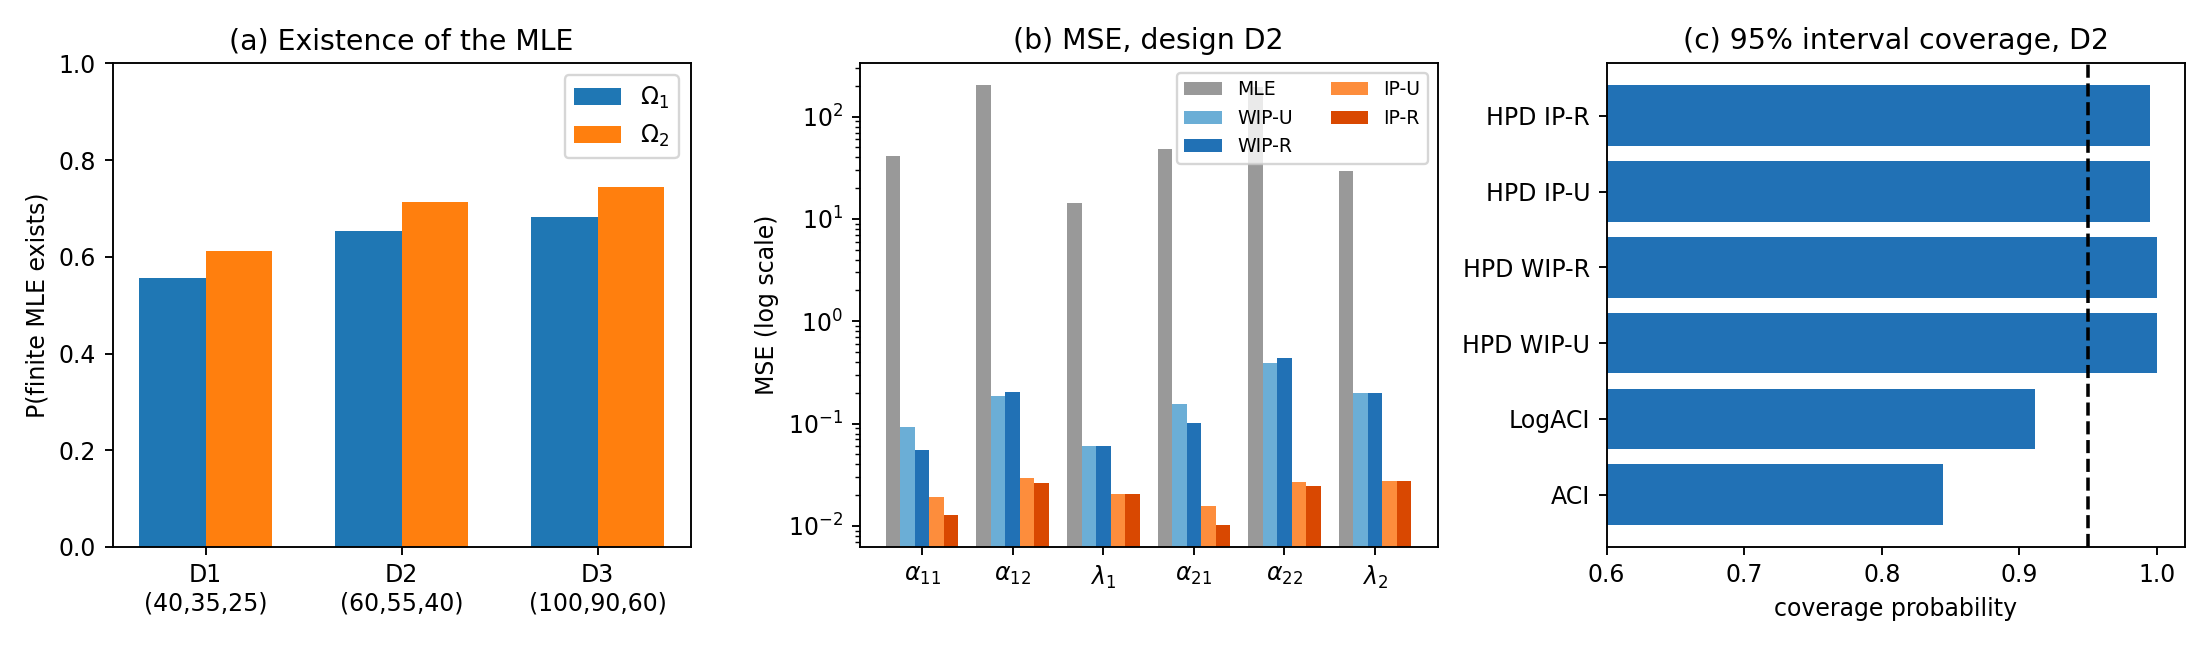
\includegraphics[width=0.95\textwidth]{fig1.png}
\caption{Simulation summary: (a) probability that a finite MLE exists; (b) MSE of MLE and Bayes (SE) estimates for D2; (c) coverage of 95\% intervals for D2 (dashed: 0.95).}\label{fig:sim}
\end{figure}

\begin{table}[htbp]
\centering\small\setlength{\tabcolsep}{4pt}
\caption{MSE of Bayes estimates under different losses, D2, unrestricted. LINEX$\pm$: $p=\pm0.5$; GE$\pm$: $q=\pm0.5$.}\label{tab:loss}
\begin{tabular}{lccccccccccc}
\hline
 & \multicolumn{5}{c}{IP} & \multicolumn{5}{c}{WIP}\\
Par. & SE & LINEX+ & LINEX$-$ & GE+ & GE$-$ & SE & LINEX+ & LINEX$-$ & GE+ & GE$-$\\\hline
$\alpha_{11}$ & 0.019 & 0.018 & 0.021 & 0.019 & 0.018 & 0.092 & 0.066 & 0.138 & 0.037 & 0.066\\
$\alpha_{12}$ & 0.029 & 0.026 & 0.036 & 0.027 & 0.027 & 0.186 & 0.102 & 0.396 & 0.067 & 0.128\\
$\lambda_1$ & 0.020 & 0.017 & 0.028 & 0.019 & 0.018 & 0.060 & 0.045 & 0.144 & 0.084 & 0.053\\
$\alpha_{21}$ & 0.016 & 0.015 & 0.017 & 0.015 & 0.015 & 0.157 & 0.118 & 0.221 & 0.062 & 0.116\\
$\alpha_{22}$ & 0.027 & 0.024 & 0.031 & 0.024 & 0.025 & 0.388 & 0.245 & 0.693 & 0.150 & 0.287\\
$\lambda_2$ & 0.028 & 0.023 & 0.042 & 0.030 & 0.025 & 0.198 & 0.272 & 0.160 & 0.446 & 0.269\\\hline
\end{tabular}
\end{table}

\begin{table}[htbp]
\centering\small\setlength{\tabcolsep}{3.5pt}
\caption{95\% intervals, D2: median width and coverage probability.}\label{tab:int}
\begin{tabular}{lcccccccccccc}
\hline
 & \multicolumn{2}{c}{ACI} & \multicolumn{2}{c}{LogACI} & \multicolumn{2}{c}{HPD WIP-U} & \multicolumn{2}{c}{HPD WIP-R} & \multicolumn{2}{c}{HPD IP-U} & \multicolumn{2}{c}{HPD IP-R}\\
Par. & width & CP & width & CP & width & CP & width & CP & width & CP & width & CP\\\hline
$\alpha_{11}$ & 1.57 & 0.75 & 3.64 & 0.90 & 1.39 & 1.00 & 1.31 & 1.00 & 0.76 & 0.99 & 0.72 & 0.99\\
$\alpha_{12}$ & 3.18 & 0.75 & 7.29 & 0.89 & 2.44 & 1.00 & 2.48 & 1.00 & 1.26 & 1.00 & 1.25 & 1.00\\
$\lambda_1$ & 10.13 & 1.00 & 47.05 & 0.92 & 2.35 & 1.00 & 2.34 & 1.00 & 1.42 & 1.00 & 1.42 & 1.00\\
$\alpha_{21}$ & 1.32 & 0.78 & 2.80 & 0.92 & 1.43 & 1.00 & 1.32 & 1.00 & 0.62 & 0.98 & 0.58 & 0.98\\
$\alpha_{22}$ & 2.62 & 0.78 & 5.22 & 0.91 & 2.49 & 1.00 & 2.53 & 1.00 & 1.02 & 1.00 & 1.01 & 1.00\\
$\lambda_2$ & 12.18 & 1.00 & 54.35 & 0.93 & 2.52 & 1.00 & 2.52 & 1.00 & 1.93 & 1.00 & 1.92 & 1.00\\\hline
\end{tabular}
\end{table}

\begin{table}[htbp]
\centering\small\setlength{\tabcolsep}{4pt}
\caption{Effect of the order restriction (D2; average over the four shape parameters): MSE of the SE Bayes estimate, median HPD width and HPD coverage, unrestricted (U) versus restricted (R).}\label{tab:restr}
\resizebox{\textwidth}{!}{\begin{tabular}{lcccccccccccc}
\hline
 & \multicolumn{6}{c}{IP} & \multicolumn{6}{c}{WIP}\\
Truth & MSE U & MSE R & wid.\ U & wid.\ R & CP U & CP R & MSE U & MSE R & wid.\ U & wid.\ R & CP U & CP R\\\hline
$\alpha_{d1}<\alpha_{d2}$ (true) & 0.023 & 0.018 & 0.92 & 0.89 & 0.99 & 0.99 & 0.206 & 0.199 & 1.94 & 1.91 & 1.00 & 1.00\\
$\alpha_{d1}=\alpha_{d2}$ (boundary) & 0.024 & 0.026 & 0.92 & 0.83 & 0.99 & 0.99 & 0.197 & 0.200 & 1.92 & 1.87 & 1.00 & 1.00\\
$\alpha_{d1}>\alpha_{d2}$ (violated) & 0.022 & 0.091 & 0.91 & 0.80 & 0.99 & 0.91 & 0.200 & 0.265 & 1.92 & 1.84 & 1.00 & 1.00\\\hline
\end{tabular}}
\end{table}

\begin{table}[htbp]
\centering\small\setlength{\tabcolsep}{3pt}
\caption{Removal pattern and thresholds (D2, true A): case frequencies I/II/III, mean $N_1/N_2$, mean probability that the MLE exists (average of $\Omega_1$ and $\Omega_2$), and average MSE over the six parameters of the SE Bayes estimates.}\label{tab:pattern}
\begin{tabular}{llcccc}
\hline
Pattern & Thr. & cases & $N_1/N_2$ & P(exist) & MSE WIP-U / IP-U\\\hline
early & PA & 0.00/0.67/0.33 & 20.6/18.6 & 0.71 & 0.180 / 0.024\\
early & PB & 0.36/0.64/0.00 & 21.3/18.7 & 0.71 & 0.187 / 0.024\\
mid & PA & 0.00/0.75/0.25 & 20.7/18.8 & 0.71 & 0.178 / 0.024\\
mid & PB & 0.49/0.51/0.00 & 21.0/19.0 & 0.71 & 0.184 / 0.024\\
late & PA & 0.01/0.99/0.00 & 20.1/19.9 & 0.64 & 0.175 / 0.022\\
late & PB & 0.96/0.04/0.00 & 20.4/19.6 & 0.62 & 0.178 / 0.022\\\hline
\end{tabular}
\end{table}

Results for D1 and D3 are in the Appendix, and all scenario-level results are in the supplementary CSV files. The main findings are the following.
\begin{enumerate}
\item \textbf{The Lomax MLE often does not exist.} A finite MLE exists in only $51$--$79\%$ of the replications across scenarios (on average $56/61\%$ in D1, $65/71\%$ in D2 and $68/75\%$ in D3 for $\Omega_1/\Omega_2$), and the probability grows only slowly with the sample size, because the condition $\Psi>0$ is about the \emph{shape} of the sample (heavy tail), not its size. When the MLE exists it is very unstable: for D2 the MSE is between $14$ and $202$ (\cref{tab:point}), because $\hat\alpha$ and $\hat\lambda$ are nearly confounded along the ridge $\alpha\lambda=$ constant; the median errors are modest, but a few estimates are huge. For the same reason the MLE's MSE does not decrease with the design size (e.g.\ $\alpha_{12}$: $111$, $202$, $397$ in D1, D2, D3).
\item \textbf{Bayes estimates with proper priors are far better.} Even the weakly informative WIP prior (mean $1$, not equal to the truth) reduces the MSE by two to three orders of magnitude (e.g.\ $\alpha_{12}$: $202$ for the MLE, $0.19$ for WIP-U). The informative prior IP is better still (MSE $0.016$--$0.029$) but is available only in simulation because it is centred at the truth. WIP is pulled towards its prior mean (AB up to $0.55$), so its error is mostly bias.
\item \textbf{Loss functions.} Differences between SE, LINEX and GE are small for IP. For WIP they follow the direction of the prior bias: since the prior mean of the $\alpha$'s ($1$) exceeds the truth, the over-estimation-averse estimators (LINEX+, GE+) have smaller MSE for $\alpha$, while for $\lambda_2$ (prior mean $1<1.5$) LINEX$-$ is best (\cref{tab:loss}). Asymmetric losses help only when the likely direction of the error is known.
\item \textbf{Intervals.} The ACI under-covers for the shapes (CP $0.75$--$0.78$) and has an absurd width for $\lambda$ (median $10$--$12$). The log-ACI is better (CP $0.89$--$0.93$) but still below $0.95$ and much wider than the HPD intervals. The HPD intervals have CP $0.98$--$1.00$: they are conservative, because both priors are centred at moderate values and the likelihood is flat (\cref{tab:int}, \cref{fig:sim}(c)). Bootstrap intervals were computed for the real data only, because $1000$ bootstrap resamples per replication were too expensive for the whole design.
\item \textbf{Order restriction.} When $\alpha_{d1}<\alpha_{d2}$ is true, the restriction changes the MSE little on average (WIP: $0.206\to0.199$; IP: $0.023\to0.018$). For IP it lowers the MSE of all four shapes, but for WIP it helps the smaller shapes and hurts the larger ones (\cref{tab:point}). When the restriction is violated, the MSE of the IP estimate quadruples ($0.022\to0.091$), the WIP MSE rises from $0.200$ to $0.265$, and the HPD coverage of IP falls from $0.99$ to $0.91$ (\cref{tab:restr}). The restriction should therefore be used only when the ordering is justified, which can be checked with the LRT of \cref{sec2} or with $P(\alpha_{d1}<\alpha_{d2}\mid\text{data})$.
\item \textbf{Censoring pattern.} Early and mid removals give practically identical results, while late removals lower the existence probability of the MLE slightly ($0.62$--$0.64$ versus $0.71$), possibly because units withdrawn late (or after $T_1$, where the adaptive rule cancels removals) carry less information about the tail; we did not test this explanation further. The Bayes MSEs hardly depend on the pattern, and the thresholds mainly change the case mix (\cref{tab:pattern}).
\end{enumerate}

\subsection{Real Data Analysis}\label{sec:real}
In this section, we present an analysis of real data for illustrative purposes.

\paragraph{Aircraft air-conditioning failures (joint design).} Proschan's \cite{proschan1963} air-conditioning failure times (hours) for Boeing 720 planes 7914 ($\Omega_1$, $m_1=24$) and 7913 ($\Omega_2$, $m_2=27$) were tabulated with the failure cause (cause 1: compressor; cause 2: all others) by Chen and Gui \cite{chen2026}. (In that table the columns are described as lifetime, population, cause, but the values only fit the reading lifetime, cause, population with 24 and 27 units per plane; we use that reading.) In $\Omega_1$ there are 15 compressor and 9 other failures; in $\Omega_2$ there are 10 and 17.

\emph{Adequacy of the Lomax model.} For the complete data the existence statistic is negative for both planes ($\Psi=-0.66$ and $-3.50$; squared coefficients of variation $0.91$ and $0.66$), so no finite MLE exists: the Lomax likelihood is maximised at the exponential limit and the data cannot distinguish a Lomax from an exponential model. The LRT of Section~\ref{sec2} for $\alpha_{d1}=\alpha_{d2}$ gives $\Lambda=1.52$ ($p=0.22$) for $\Omega_1$ (counts $15/9$) and $\Lambda=1.84$ ($p=0.18$) for $\Omega_2$ (counts $10/17$): the two cause-specific shapes are not significantly different.

\emph{JIAPCS applied to the data.} We applied the scheme with $k=18$, $R_8=R_9=3$ (all other $R_i=0$; $\sum(R_i+1)=23<24$), $T_1=0.45$, $T_2=1.8$; the withdrawn units are chosen at random from the survivors. Over 200 random withdrawal patterns a finite MLE existed for $\Omega_1$ in $47\%$ and for $\Omega_2$ in $20\%$ of the patterns, and for both in only $5.5\%$. To illustrate the full procedure we report the first pattern (random seed 40) for which both MLEs exist; this is an \emph{atypical} sample chosen for illustration (Case II, 18 failures: $\Omega_1$ with $N=10$, causes $5/5$; $\Omega_2$ with $N=8$, causes $6/2$). Results are in \cref{tab:air} and \cref{fig:real1}.

\begin{table}[htbp]
\centering\small\setlength{\tabcolsep}{5pt}
\caption{Aircraft data (one JIAPCS sample). MLE, restricted MLE (R), bootstrap-p 95\% interval, and Bayes estimates under the WIP prior: SE, LINEX ($p=0.5$), GE ($q=0.5$) with 95\% HPD interval, and the restricted SE estimate with HPD.}\label{tab:air}
\begin{tabular}{lcccccccccc}
\hline
Par. & MLE & MLE-R & Boot-p & SE & LINEX & GE & HPD & SE-R & HPD-R\\\hline
$\alpha_{11}$ & 1.631 & 1.631 & [0.10, 11.59] & 1.118 & 1.018 & 0.857 & [0.19, 2.50] & 0.875 & [0.15, 1.84]\\
$\alpha_{12}$ & 1.631 & 1.631 & [0.08, 11.70] & 1.107 & 1.008 & 0.847 & [0.17, 2.50] & 1.378 & [0.33, 2.85]\\
$\lambda_1$ & 0.539 & 0.539 & [0.06, 19.44] & 1.109 & 0.999 & 0.834 & [0.17, 2.50] & 1.060 & [0.19, 2.42]\\
$\alpha_{21}$ & 0.946 & 0.630 & [0.06, 8.11] & 1.205 & 1.076 & 0.902 & [0.18, 2.82] & 0.763 & [0.10, 1.70]\\
$\alpha_{22}$ & 0.315 & 0.630 & [0.03, 3.46] & 0.520 & 0.480 & 0.328 & [0.03, 1.33] & 1.028 & [0.17, 2.32]\\
$\lambda_2$ & 0.762 & 0.762 & [0.08, 36.57] & 0.834 & 0.749 & 0.567 & [0.06, 2.03] & 0.799 & [0.08, 2.03]\\\hline
\end{tabular}
\end{table}

\begin{figure}[htbp]
\centering
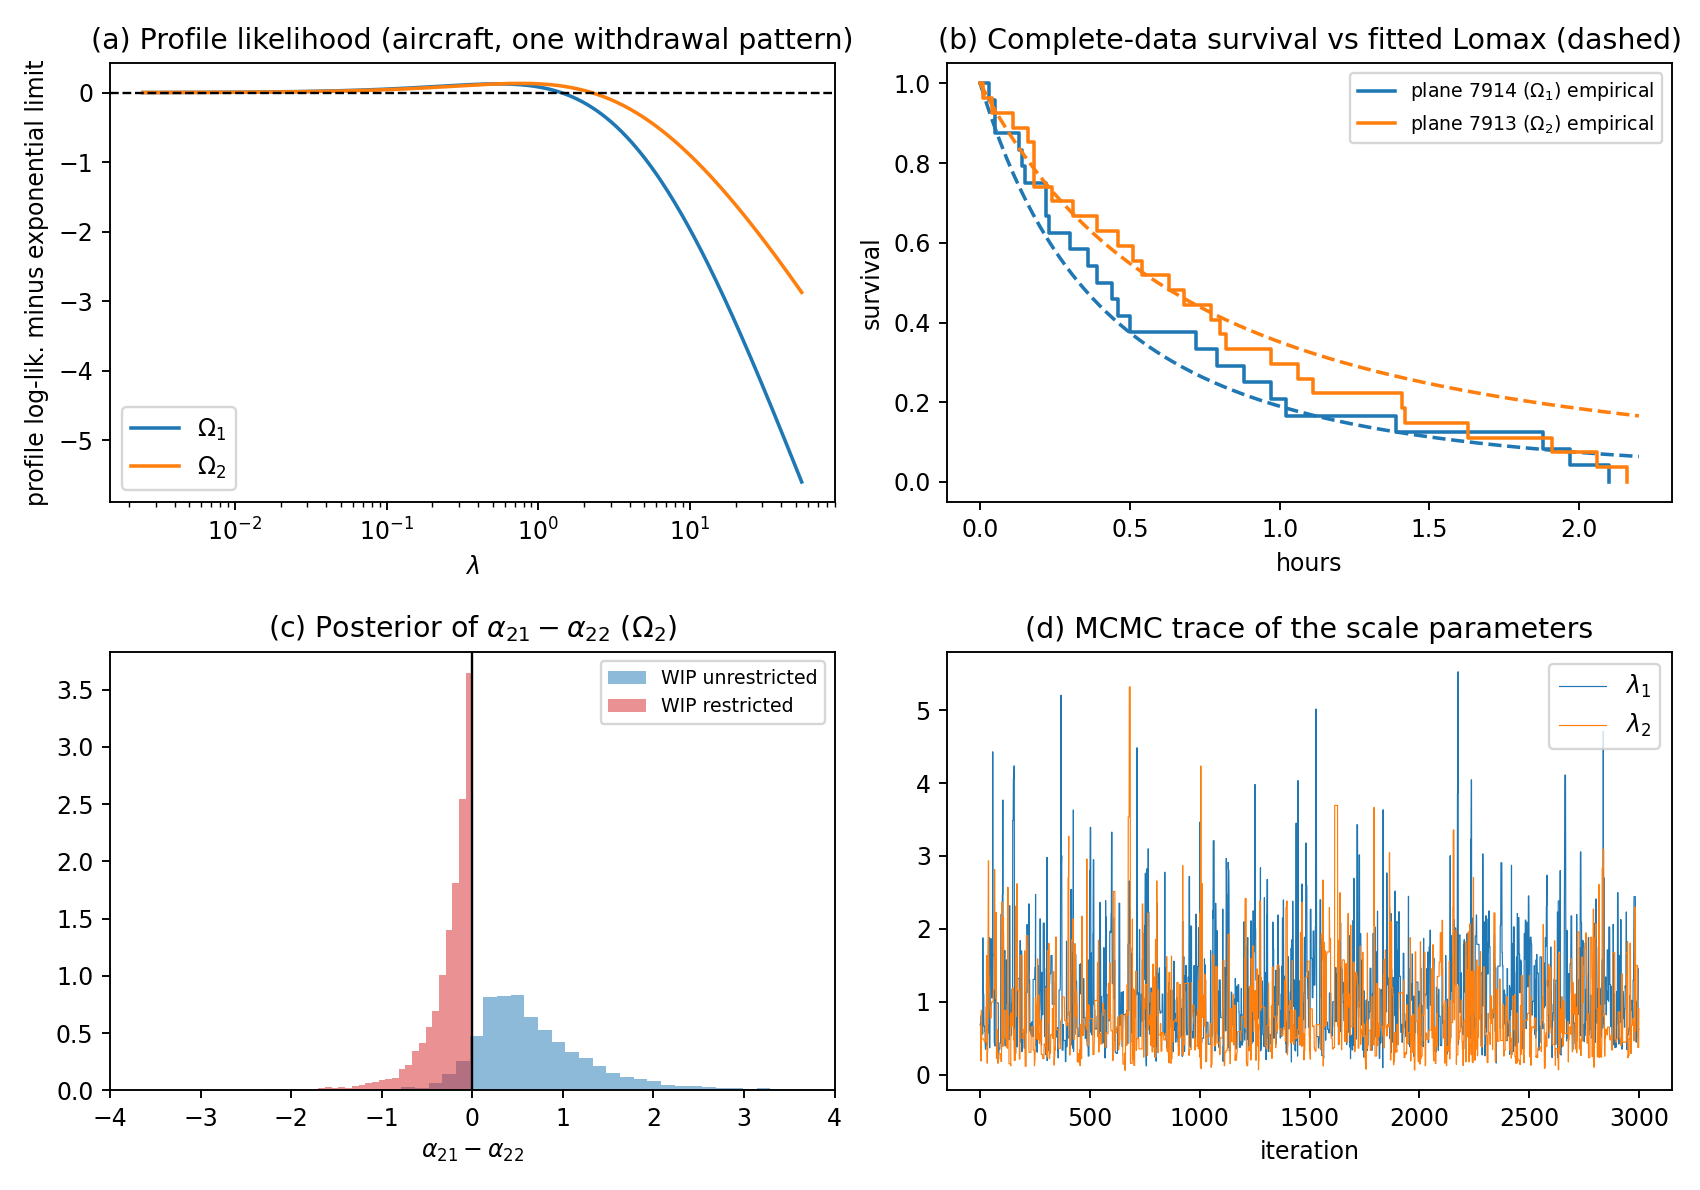
\includegraphics[width=0.78\textwidth]{fig2.png}
\caption{Aircraft data: (a) profile log-likelihood relative to the exponential limit; (b) empirical survival functions of the complete samples and fitted Lomax curves; (c) posterior of $\alpha_{21}-\alpha_{22}$; (d) MCMC traces of $\lambda_1,\lambda_2$.}\label{fig:real1}
\end{figure}

\emph{Findings.} (i) The profile log-likelihood exceeds its exponential-limit value by only $0.13$ for both populations (\cref{fig:real1}(a)). As an LRT of ``exponential'' against ``Lomax'' this is $2\times0.13=0.26$; since the exponential model sits on the boundary ($\alpha\to\infty$), the null distribution is the mixture $\tfrac12\chi^2_0+\tfrac12\chi^2_1$ and the approximate $p$-value is $\tfrac12P(\chi^2_1>0.26)\approx0.31$. There is no evidence for a Lomax shape. (ii) The bootstrap-p intervals are extremely wide (e.g.\ $\lambda_1$: $[0.06,19.4]$) and only $52\%$ and $45\%$ of the bootstrap samples had a finite MLE. (iii) The Bayes estimates are close to the prior means (WIP has mean $1$), so the data hardly update the prior; the HPD intervals are wide. (iv) In this particular censored sample $\Omega_2$ has $6$ failures of cause 1 and only $2$ of cause 2, so the unrestricted posterior gives $P(\alpha_{21}<\alpha_{22}\mid\text{data})=0.09$, whereas in the complete data cause 2 is more frequent ($17$ versus $10$). The restricted estimate simply imposes the ordering, which shows why the restriction should be checked and why very small samples cannot support it. (v) The fitted Lomax curves follow the empirical survival curves reasonably well (\cref{fig:real1}(b)), as they must when the model is close to exponential.

\paragraph{Electrical appliances (single-population analysis).} Because the aircraft data are near-exponential, we also used a data set with a clearly decreasing early failure rate: the 36 small electrical appliances of Lawless \cite{lawless2003}, in the improved-adaptive competing risks form used in the literature (see \cite{alotaibi2025}). The first 16 failures ($n=36$) occurred at times $11,35,49,170,\dots,2400$ (we divided by $1000$) and the remaining 20 units were withdrawn at the last failure, i.e.\ $\nu=(1,\dots,1,21)$. Cause 2 is failure mode 9 (10 failures) and cause 1 collects all other modes (6 failures); the labels are chosen so that $\alpha_1\le\alpha_2$ is the plausible ordering. Since the likelihood factorises by population, this analysis uses exactly the same estimators (a JIAPCS in which only one population is observed); we do \emph{not} claim a joint analysis here. Results are in \cref{tab:app} and \cref{fig:real2}.

\begin{table}[htbp]
\centering\small\setlength{\tabcolsep}{2.5pt}
\caption{Appliance data: estimates as in \cref{tab:air}.}\label{tab:app}
\begin{tabular}{lccccccccc}
\hline
Par. & MLE & MLE-R & Boot-p & SE & LINEX & GE & HPD & SE-R & HPD-R\\\hline
$\alpha_1$ & 0.602 & 0.602 & [0.08, 6.54] & 0.533 & 0.490 & 0.352 & [0.05, 1.39] & 0.463 & [0.05, 1.20]\\
$\alpha_2$ & 1.004 & 1.004 & [0.14, 10.18] & 0.831 & 0.747 & 0.577 & [0.10, 2.09] & 0.844 & [0.12, 2.13]\\
$\lambda$ & 0.181 & 0.181 & [0.01, 2.90] & 0.471 & 0.422 & 0.260 & [0.02, 1.39] & 0.489 & [0.04, 1.51]\\\hline
\end{tabular}
\end{table}

\begin{figure}[htbp]
\centering
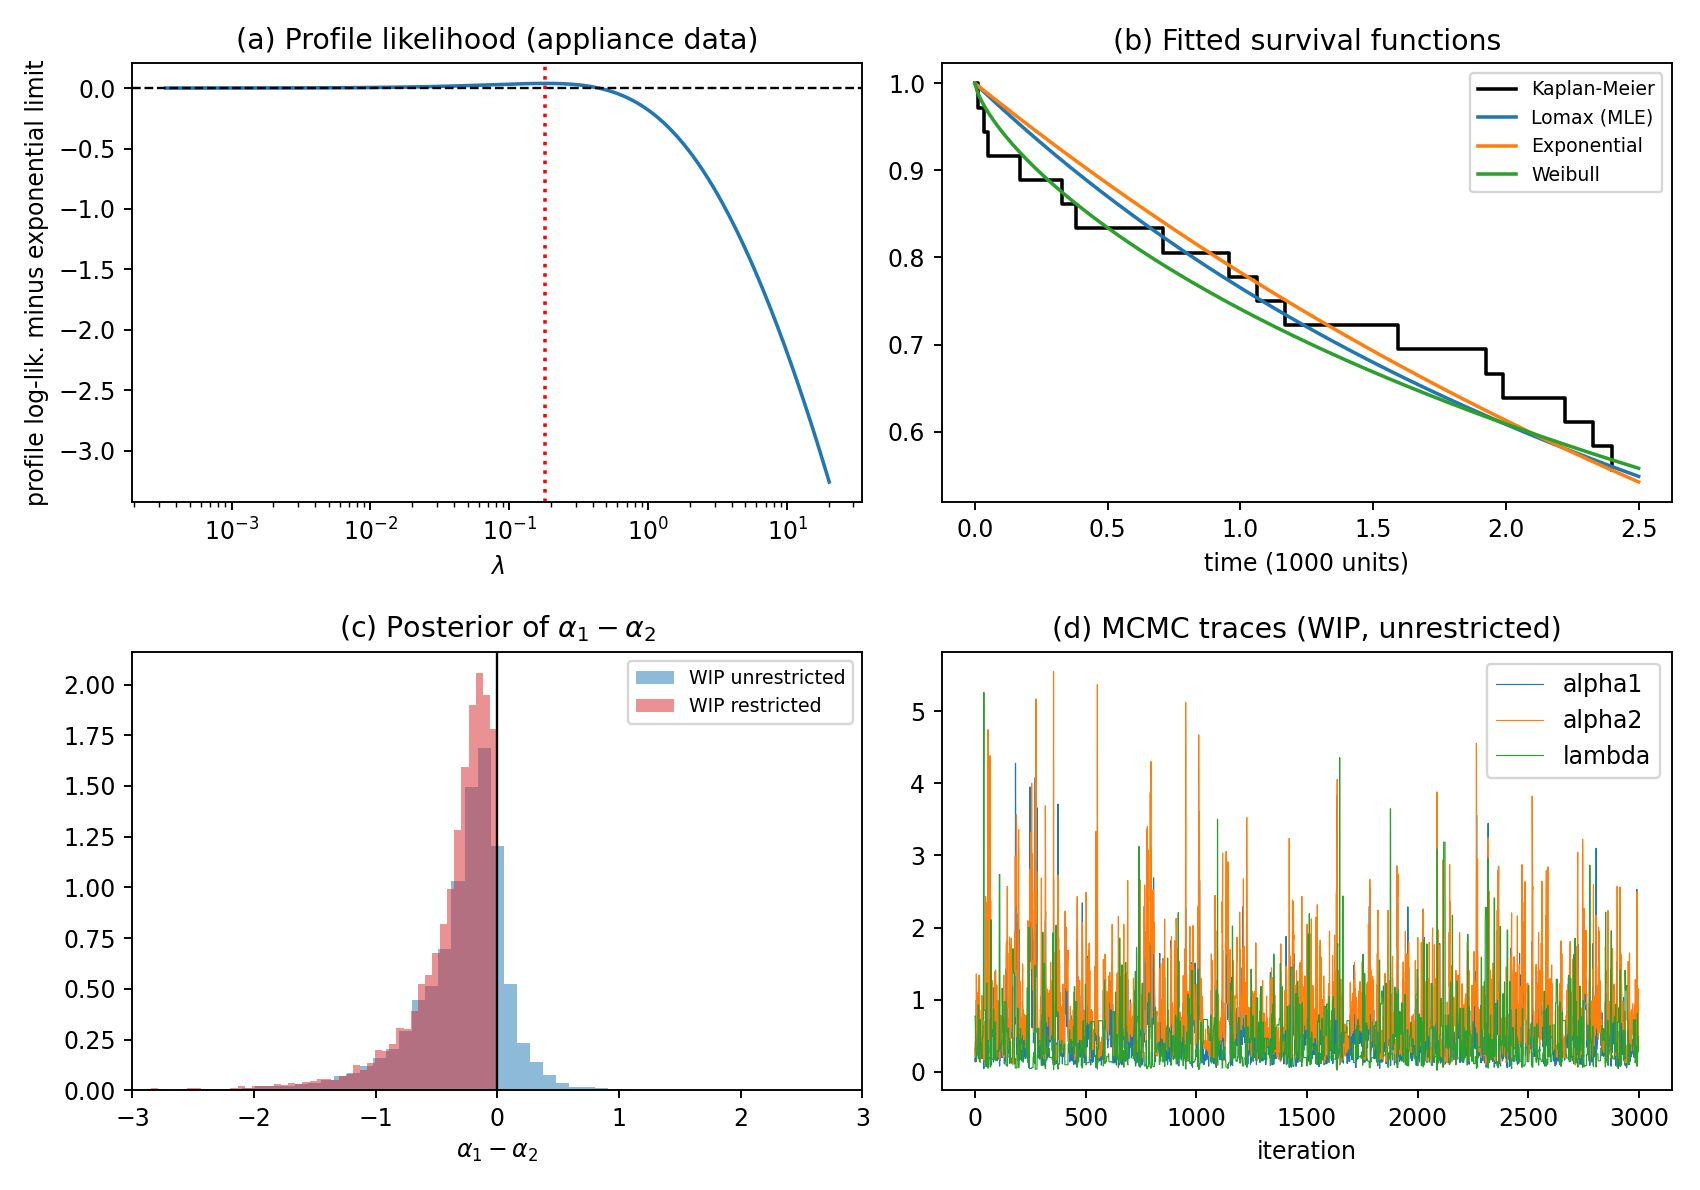
\includegraphics[width=0.78\textwidth]{fig3.png}
\caption{Appliance data: (a) profile log-likelihood relative to the exponential limit (dotted: MLE); (b) Kaplan--Meier curve and fitted survival functions; (c) posterior of $\alpha_1-\alpha_2$; (d) MCMC traces.}\label{fig:real2}
\end{figure}

\emph{Findings.} Here $\Psi=0.52>0$ and the MLE exists: $\hat\alpha=(0.602,1.004)$, $\hat\lambda=0.181$. (i) The asymptotic intervals are useless (ACI for $\alpha_1$: $[-3.7,4.9]$; log-ACI: $[0.0005,763]$), confirming the simulation; the bootstrap-p intervals are wide but sensible, and only $47\%$ of the bootstrap samples had a finite MLE. (ii) Ignoring the cause labels, the censored log-likelihoods of the lifetime distribution are $-38.47$ (Lomax, 2 parameters), $-38.51$ (exponential, 1) and $-37.48$ (Weibull, 2), so the AICs are $80.9$, $79.0$ and $79.0$. The Lomax therefore gives no real improvement over the exponential and is not preferred by AIC, although all three curves follow the Kaplan--Meier curve closely (\cref{fig:real2}(b)). The LRT against the exponential gives $2\times0.04\approx0.08$ and an approximate boundary $p$-value of about $0.39$. (iii) The WIP posterior (SE) is $(0.533,0.831,0.471)$ and a Gamma$(2,2)$ prior gives nearly the same $(0.497,0.749,0.425)$, whereas the NIP prior gives posterior means of $\alpha$ of $40.7$ and $70.7$ (Remark~\ref{rem:nip} in action). (iv) $P(\alpha_1<\alpha_2\mid\text{data})=0.83$, so the restriction is plausible but not strongly supported, and the restricted and unrestricted estimates are close.

\section{Conclusion}\label{sec6}
In this paper, we develop classical and Bayesian estimators of the Lomax competing risks model under the joint improved adaptive progressive censoring scheme. The likelihood factorises by population, the shapes have closed-form conditional MLEs, the order-restricted MLE is obtained by pooling, and a collapsed sampler gives exact Bayes estimates for the unrestricted and the order-restricted prior. Our main conclusions are:
\begin{itemize}
\item The Lomax MLE exists only when the sample is heavy-tailed enough ($\Psi>0$); otherwise the data support the exponential limit. A finite MLE existed in only $51$--$79\%$ of simulated samples and was very unstable, so its existence should always be checked before it is reported.
\item Bayes estimates with proper (even weakly informative) priors are much more accurate and always exist; vague priors with tiny hyperparameters must be avoided for this model.
\item Asymptotic intervals under-cover; HPD intervals are shorter and conservative.
\item The order restriction is useful only if it is true; its plausibility can be checked with the likelihood ratio test or the posterior probability of the ordering.
\item Both real data sets were close to exponential, so they illustrate the procedures but cannot confirm a Lomax shape.
\end{itemize}
\textbf{Limitations.} We assumed a common $\lambda_d$ for the two causes within a population and independent latent lifetimes; the simulation uses one configuration of true values; the informative prior is centred at the truth and is therefore optimistic; the MLE is evaluated only on the samples where it exists; the bootstrap intervals were not part of the simulation study; uniqueness of $\hat\lambda$ was checked numerically, not proved; and the aircraft illustration uses a rare withdrawal pattern. Natural extensions are different scale parameters for the two causes, bootstrap-t intervals, optimal choice of the censoring scheme, and dependent causes.

\appendix
\section{Results for designs D1 and D3}
\begin{table}[htbp]
\centering\small\setlength{\tabcolsep}{4pt}
\caption{Point estimation, design D1 (same layout as \cref{tab:point}).}
\begin{tabular}{lcccccccccccc}
\hline
 & \multicolumn{2}{c}{MLE} & \multicolumn{2}{c}{WIP-U} & \multicolumn{2}{c}{WIP-R} & \multicolumn{2}{c}{IP-U} & \multicolumn{2}{c}{IP-R}\\
Parameter (true) & med.\ err. & MSE & AB & MSE & AB & MSE & AB & MSE & AB & MSE\\\hline
$\alpha_{11}$ (0.5) & $-0.23$ & 118.2 & 0.229 & 0.112 & 0.144 & 0.050 & 0.024 & 0.022 & 0.013 & 0.013\\
$\alpha_{12}$ (1.0) & $-0.45$ & 111.2 & 0.311 & 0.182 & 0.397 & 0.215 & 0.041 & 0.034 & 0.078 & 0.030\\
$\lambda_1$ (1.0) & $+1.21$ & 54.8 & 0.035 & 0.053 & 0.034 & 0.054 & 0.051 & 0.025 & 0.051 & 0.025\\
$\alpha_{21}$ (0.4) & $-0.17$ & 44.1 & 0.349 & 0.188 & 0.248 & 0.093 & 0.019 & 0.018 & 0.018 & 0.011\\
$\alpha_{22}$ (0.8) & $-0.33$ & 291.5 & 0.536 & 0.384 & 0.637 & 0.468 & 0.037 & 0.032 & 0.074 & 0.029\\
$\lambda_2$ (1.5) & $+1.44$ & 186.8 & 0.375 & 0.200 & 0.375 & 0.200 & 0.042 & 0.030 & 0.042 & 0.030\\\hline
\end{tabular}
\end{table}
\begin{table}[htbp]
\centering\small\setlength{\tabcolsep}{4pt}
\caption{Point estimation, design D3.}
\begin{tabular}{lcccccccccccc}
\hline
 & \multicolumn{2}{c}{MLE} & \multicolumn{2}{c}{WIP-U} & \multicolumn{2}{c}{WIP-R} & \multicolumn{2}{c}{IP-U} & \multicolumn{2}{c}{IP-R}\\
Parameter (true) & med.\ err. & MSE & AB & MSE & AB & MSE & AB & MSE & AB & MSE\\\hline
$\alpha_{11}$ (0.5) & $-0.15$ & 85.8 & 0.200 & 0.078 & 0.172 & 0.057 & 0.023 & 0.015 & 0.009 & 0.011\\
$\alpha_{12}$ (1.0) & $-0.28$ & 397.3 & 0.339 & 0.185 & 0.367 & 0.196 & 0.047 & 0.024 & 0.062 & 0.022\\
$\lambda_1$ (1.0) & $+0.54$ & 7.48 & 0.028 & 0.063 & 0.028 & 0.063 & 0.054 & 0.018 & 0.054 & 0.018\\
$\alpha_{21}$ (0.4) & $-0.10$ & 24.8 & 0.305 & 0.135 & 0.271 & 0.103 & 0.019 & 0.012 & 0.004 & 0.009\\
$\alpha_{22}$ (0.8) & $-0.19$ & 85.3 & 0.550 & 0.377 & 0.583 & 0.404 & 0.043 & 0.021 & 0.057 & 0.019\\
$\lambda_2$ (1.5) & $+0.65$ & 13.1 & 0.349 & 0.193 & 0.349 & 0.193 & 0.046 & 0.025 & 0.047 & 0.025\\\hline
\end{tabular}
\end{table}

%\newpage
\bibliographystyle{IEEEtran}
\bibliography{reference}

\end{document}
